\documentclass[a4paper]{article}
\usepackage[utf8]{inputenc}
\usepackage{fancyhdr}
\usepackage{geometry}
\usepackage{listings}
\usepackage{graphicx}
\usepackage{algorithmic}
%\geometry{0.5in}

\usepackage{float}

\lstset{
    language=Python,
    breaklines=true,
    numbers=left,
    frame=lines
}

\pagestyle{fancyplain}

\title{System Maintenance}
\author{Harry Milne}
\date{March 2014}

\lhead{Harry Milne}
\chead{Candidate Number: 2677}
\rhead{Centre Number: 22169}

\begin{document}
\maketitle
\tableofcontents


\section{Environment}
    \label{sec:env}
    \subsection{Software}
    \begin{itemize}
        \item Python 2.7 and included modules
        
        \begin{itemize}
            \item SQLite3
        \end{itemize}
        
        \item Twisted 13.2.0 Python Module
        \item PyQt4 Python Module
        \item SimpleCV 1.3
        \item SQLite Database Browser
        \item Vim
        \item Sublime Text 3
    \end{itemize}

    \begin{table}[H]
        \centering
        \begin{tabular}{|p{4cm}|p{8cm}|}
        \hline
        \textbf{Software}                & \textbf{Usage Explanation}                                                                                                                                                                                            \\ \hline
        Python 2.7              & I used Python 2.7 instead of Python 3.* because of the superior module support that Python 2.5+ has. Also, the nature of Python itself makes it very easy to build systems quickly.                          \\ \hline
        SQLite3                 & SQLite3 was an easy database management system to use because it has little requirements for the system it is run on. This means you do not have to do any extensive configuration of any target system.      \\ \hline
        Twisted 13.2.0          & Twisted is a Python module which lets you very quickly prototype and build clients and servers, which is central to this system.                                                                             \\ \hline
        PyQt4                   & PyQt4 is a feature rich user interface development module, it handles all of the threading needed to run operations while keeping an operational interface.                                                  \\ \hline
        SimpleCV 1.3            & SimpleCV is aimed at making computer vision easy to develop, I used it in conjunction with the Raspberry Pi to recognise faces.                                                                              \\ \hline
        SQLite Database Browser & This open source software gives an easy way to visually check over your SQLite databases, this was invaluable in testing.                                                                                    \\ \hline
        Vim                     & When developing the python server script, it was easier to program it while on the server itself instead of deploying to it every time I wanted to test. This meant using a text editor that works in shell. \\ \hline
        Sublime Text 3          & This was the editor of choice while programming in a GUI environment, it has a lot of tools to help with syntax highlighting and variable naming.                                                            \\ \hline
        \end{tabular}
    \end{table}


\section{System Overview}
The system has 3 main components; the client, server and database browser. The server and client are directly related
whereas the database browser is a `tool' I have bundled to help the user manage the database. The database browser works
with the server on a local level, in that you edit the same file on the same system that the server does. However,
the database browser requires the server to be running a graphical user environment because it is a graphical representation
of the database. 

    \subsection{Client}
    The client uses the SimpleCV package as shown in section~\ref{sec:env}, this package handles everything around the camera,
    this makes it easier to read what is happening with the data being handled by the Python. The client package needs to be
    running everywhere where you want to be able to toggle the alarm system. 

    \subsection{Server}
    The server will be installed on a dedicated computer which will not be turned off, the Python script runs as a daemon
    which the Twisted Python package (section~\ref{sec:env})) handles. The server can be set up to use whatever port is defined
    in the configuration file, as mentioned in section~\ref{sec:settings}, this should be the exact same number as every client
    uses.

    The server needs to be running for the client to interact with the alarm system, otherwise the client will receive network
    errors.

    \subsection{Database Browser}
    The database browser gives the system administrator an easy interface to edit the database, this is required for
    adding new users to the system. Once the client and server are set up with the same users the system will work
    correctly. Unfortunately there was no easy way to set up the system to update every single node whenever a user is
    added, so this tool is necessary for the system to work.


\section{Code Structure}
I structured the code so that each section of the system was an object, abstracting like this helps a lot with
visualising the code. By doing this I have taken one of the advantage of object-oriented programming; the ability
to abstract certain situations into particular `objects'.

    \subsection{Client Class}
    \label{sec:clientstructure}
    The class created in `client.py', which can be found in section~\ref{sec:client.py}, includes methods to handle
    the processing of images that it will be continuously scanning. 

    The code is laid out so that the face recognition methods and networking methods are physically separated, this means
    coming back to file file isn't a lot of scrolling trying to find the appropriate functions, instead they are somewhat
    ordered.

    The most prominent method in the `Client' class is the `start' method, this triggers the client to start processing
    images from the given camera. This loop is purposely infinite because it is a daemon and doesn't need to `finish', unlike
    most conventional code where the code has an `end' state, this just loops until a `KeyboardInterrupt' is triggered.

    \lstinputlisting[language=Python, 
                    firstline=36, 
                    lastline=47,
                    label={lst:clientstart},
                    caption=The start method from section~\ref{sec:client.py}.]{../../code/client/client.py}

    \subsection{Handler Class}
    The server class created in `server.py' is called `Handler' as shown in section~\ref{sec:server.py} line 8, this is 
    because it `handles' the requests from the client. Inside this class there is an `SQLInterface' instantiation to give 
    the server an interface for the `SQLite3' database, however, methods that edit the database will only be run after the 
    server knows the user trying to access it is already in it. Unfortunately, there is no other security around authenticating 
    users, the only barrier between someone sending a string to the server and gaining access is that they don't know the users 
    already in the database.

    \subsection{SQLInterface Class}
    I structured it this way so that if one needed to access the database from another Python script, they'd
    have a standardised method of doing so. This means they can simply import the package and either instantiate it `as is'
    or use it as a parent class to add functionality. This way of modular programming is much appreciated by many a programmer,
    as it means you don't have to scrawl through existing code to find where the SQL statements had been `hard-coded' into the
    main program, instead of separating the functions which interfaced with the database.

    \subsection{Database Browser}
    Here I didn't choose the layout of the code, because it was a cloned open sourced repository from GitHub.
    However, when editing the code I stuck to the same format as the previous programmer as to keep the consistency; this
    means using the same naming convention and using same methods where appropriate.

\section{Variable Listing}

\begin{table}[H]
    \begin{tabular}{|l|l|l|l|}
    \hline
    Variable Name & Purpose                                            & Section                   & Line Number \\ \hline
    cam           & Store Camera object                                & \ref{sec:client.py} & 12          \\ \hline
    cfg           & Store Config                                       & \ref{sec:client.py} & 20          \\ \hline
    host          & Hold host IP for future reference                  & \ref{sec:client.py} & 22          \\ \hline
    host\_port    & Host port for future reference                     & \ref{sec:client.py} & 23          \\ \hline
    haar\_path    & Path to Haar Cascade XML file                      & \ref{sec:client.py} & 24          \\ \hline
    data\_con     & List of data directory                             & \ref{sec:client.py} & 28          \\ \hline
    face          & Face of user object                                & \ref{sec:client.py} & 39          \\ \hline
    result        & Match object of matched face                       & \ref{sec:client.py} & 43          \\ \hline
    img           & Image from camera                                  & \ref{sec:client.py} & 51          \\ \hline
    faces         & List of detected faces                             & \ref{sec:client.py} & 52          \\ \hline
    usr\_list     & List of users defined                              & \ref{sec:client.py} & 61          \\ \hline
    result\_list  & List of face matches                               & \ref{sec:client.py} & 68          \\ \hline
    s             & Socket object                                      & \ref{sec:client.py} & 87          \\ \hline
    c             & Client object                                      & \ref{sec:client.py} & 104         \\ \hline
    menu\_bar     & ~                                                  & \ref{sec:dbbrowser.py} & 21          \\ \hline
    menu\_new     & Menu for new object list                           & \ref{sec:dbbrowser.py} & 24          \\ \hline
    tab\_data     & QWidget defined for browsing data                  & \ref{sec:dbbrowser.py} & 39          \\ \hline
    layout        & QWidget for ordering QWidgets in a vertical layout & \ref{sec:dbbrowser.py} & 45          \\ \hline
    db\_connection & Database connection object                         & \ref{sec:dbbrowser.py} & 74          \\ \hline
    parent        & Reference to parent object                         & \ref{sec:server.py} & 11          \\ \hline
    sql           & SQLInterface instantiation                         & \ref{sec:server.py} & 12          \\ \hline
    peer          & Contains data about connected client               & \ref{sec:server.py} & 22          \\ \hline
    data          & Data received from client                          & \ref{sec:server.py} & 25          \\ \hline
    data\_list    & Data from client split by whitespace               & \ref{sec:server.py} & 27          \\ \hline
    STATE         & Current alarm state                                & \ref{sec:server.py} & 48          \\ \hline
    db\_fname     & Database file name                                 & \ref{sec:sqlinterface.py} & 14          \\ \hline
    log\_path     & Path to log file                                   & \ref{sec:sqlinterface.py} & 19          \\ \hline
    table\_queries & List of table creation SQL statements              & \ref{sec:sqlinterface.py} & 34          \\ \hline
    on\_off       & List with index 0 at OFF and index 1 at ON         & \ref{sec:sqlinterface.py} & 117         \\ \hline
    log\_f        & Log file                                           & \ref{sec:sqlinterface.py} & 122         \\ \hline
    db            & SQLInterface instantiation                         & \ref{sec:sqlinterface.py} & 133         \\ \hline
    \end{tabular}
\end{table}

\section{System Evidence}
    \subsection{User Interface}
    \subsection{ER Diagram}
    \begin{figure}[H]
        \caption{Entity Relationship Diagram of the SQLite database.}
        \centering
        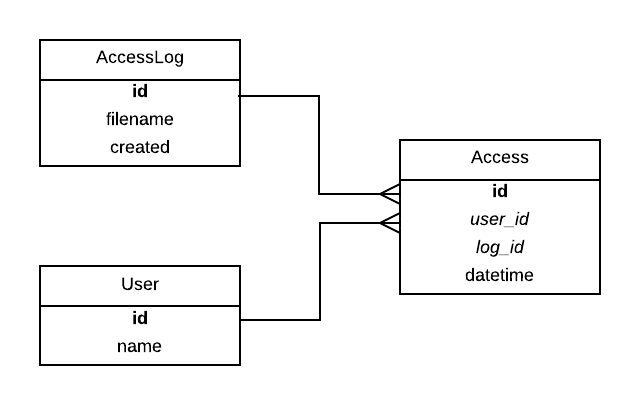
\includegraphics[scale=0.3]{../shared_assets/diagrams/ERD.png}
    \end{figure}

    \subsection{Database Table Views}
        \subsubsection{Users}
            \begin{figure}[H]
                \caption{Screenshot of the Users table in the database.}
                \centering
                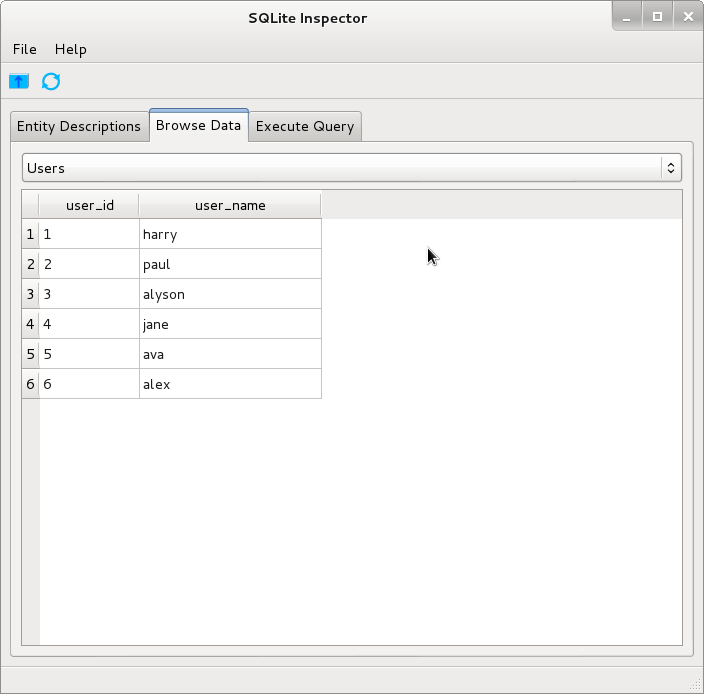
\includegraphics[scale=0.5]{../shared_assets/screenshots/database_users.png}
            \end{figure}

        \subsubsection{Access}
            \begin{figure}[H]
                \caption{Screenshot of the Access table in the database.}
                \centering
                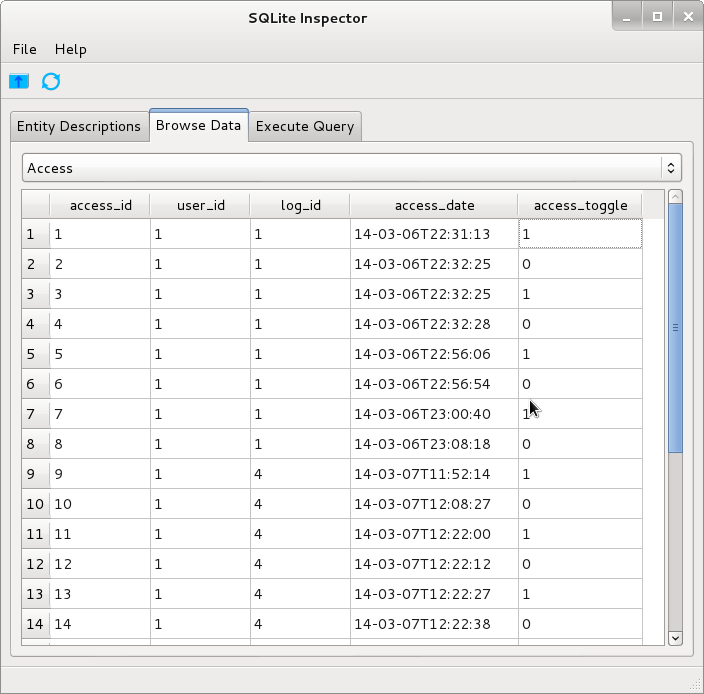
\includegraphics[scale=0.5]{../shared_assets/screenshots/database_access.png}
            \end{figure}

        \subsubsection{Log}
            \begin{figure}[H]
                \caption{Screenshot of the Log table in the database.}
                \centering
                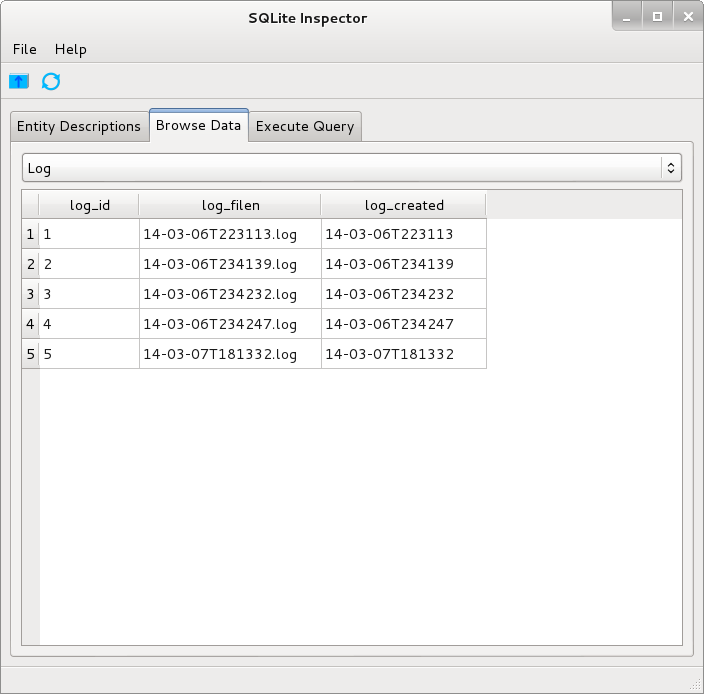
\includegraphics[scale=0.5]{../shared_assets/screenshots/database_log.png}
            \end{figure}

        \newpage
        \subsection{Database SQL}

        \lstinputlisting[language=Python, 
                        firstline=32, 
                        lastline=56,
                        label={lst:createtables},
                        caption=Extract from sql\_interface.py]{../../code/server/sql_interface.py}
        Above, in Listing~\ref{lst:createtables}, you can see the function inside the `SQLInterface' class which creates the tables
        within the database. This function \textit{must} be ran before any other inside the class if the database
        hasn't been initialised before, otherwise an exception will be thrown saying either that the database 
        doesn't exist yet or the tables don't exist.

        The structure of this function has been coded with the `DRY' (`Don't Repeat Yourself') principle in mind;
        instead of running each SQL statement individually, the strings are in a list which can be iterated over.

    \subsection{SQL Queries}

    \begin{table}[H]
        \centering
        \begin{tabular}{|p{5cm}|p{8cm}|}
        \hline
        \textbf{Functionality}                                                                                                                   & \textbf{SQL Statement}                                                                                                                                          \\ \hline
        Creates a new User with the given user\_name.                                                                   & INSERT INTO Users(user\_name) values (?)                                         \\ \hline
        Delete a user with a given id.                                                                                  & DELETE FROM Users where user\_id = ?                                             \\ \hline
        Return all stored user\_name attributes in the Users table.                                                     & SELECT user\_name FROM Users                                                     \\ \hline
        Return all Users entities with the given user\_name.                                                            & SELECT * from Users WHERE user\_name = ?                                         \\ \hline
        Return the Users entity with the given user\_id.                                                                & SELECT user\_name FROM Users WHERE user\_id = ?                                  \\ \hline
        Create new Log entity with the given filename and created date.                                                 & INSERT INTO Log(log\_filen, log\_created) VALUES (?,?)                           \\ \hline
        Return the Log with the highest id number.                                                                      & SELECT * FROM Log WHERE log\_id=(SELECT MAX(log\_id) FROM Log)                   \\ \hline
        Create an entity in the Access table with the given attributes; user\_id, log\_id, access\_date and access\_toggle. & INSERT INTO Access(user\_id, log\_id, access\_date, access\_toggle) VALUES (?,?,?,?) \\ \hline
        Return all Access entities initiated with the given user\_id.                                                   & SELECT * FROM Access WHERE user\_id = ?                                          \\ \hline
        \end{tabular}
    \end{table}

\section{Testing}
    \subsection{Summary of Results}
        The results of testing, as shown in the `Testing' document, show that the code is for the most part empty of bugs. However, this
        has come at the cost of losing a few features, for example, the database browser doesn't include all of the features shown in the 
        design mock-ups of the user interface.

        Things that testing did show was that the system isn't easy to set up, luckily my intended client has an extensive knowledge of
        computer systems, he works as a CTO (Chief Technology Officer) and previously has had experience with programming languages such as
        C++ and Fortran 77.
    \subsection{Known Issues}
        Issues with this system are mostly security and set-up based, in it's current state it is very hard to keep the whole system running
        with each node up to date. 

        Some of the issues include:
        \begin{itemize}
            \item Server security
            \item Ease of Set-up
            \item System-wide Database updates
        \end{itemize}

\section{Code Explanations}
    \subsection{Difficult Sections}
        \subsubsection{Client}

        The below method, listing~\ref{lst:getcfg}, shows the method which is used to parse the configuration file for the client. First, on line 2,
        Python checks to see if `client.cfg' exists before running the rest of the code, if it doesn't, nothing will be parsed. On line 3 the function
        instantiates a `ConfigParser', which is a package which is included with Python. This is used as an abstraction of the configuration file, you
        read the file in on line 4. The last 3 lines are retrieving settings from the abstraction of the configuration file and setting them as attributes
        of the Client object. This is done so that these settings can be read from other functions without explicitly passing them.

        \begin{figure}[H]
        \lstinputlisting[language=Python, 
                        firstline=18, 
                        lastline=24,
                        label={lst:getcfg},
                        caption=get\_cfg method from section~\ref{sec:client.py}]{../../code/client/client.py}
        \end{figure}

        Listing~\ref{lst:clientstart} in section~\ref{sec:clientstructure} shows the start method of the Client class, on line 3 a infinite loop is started because we want to run this script
        as a daemon. Line 4 we retrieve a face from the camera and store the return value in the `face' variable, if a face wasn't detected the face variable
        will be equal to None, otherwise it will be an object from SimpleCV. Once a face is detected, line 7 will let the rest of the code run, so we can then
        check if it matches any of the stored faces in the client data folder. This works the same in that if it doesn't return a match result will equal None,
        so if it is a success it will fall through to line 10 where we send a packet to the server requesting an alarm toggle.

        \subsubsection{Server}

        \lstinputlisting[language=Python, 
                        firstline=25, 
                        lastline=41,
                        label={lst:linereceived},
                        caption=lineRecieved method from section~\ref{sec:server.py}]{../../code/server/server.py}

        The function in listing~\ref{lst:linereceived} is called as part of the Twisted package, when a string is received with the given delimiter this method is called. Here we are passed the
        data from the line which has been received, so we check if it is a valid request. The data is split by the white space so we can number the arguments, then
        we run through and check to see if these arguments are valid. If any of them are incorrect we will end the connection with the client and return them a string
        stating that it failed.

        \subsubsection{SQLInterface}

        \lstinputlisting[language=Python, 
                        firstline=112, 
                        lastline=123,
                        label={lst:logaccess},
                        caption=log\_access method from section~\ref{sec:sqlinterface.py}]{../../code/server/sql_interface.py}

        Listing~\ref{lst:logaccess} shows a very dense method from the SQLInterface class in section~\ref{sec:sqlinterface.py}, this is because it needs to handle two things;
        appending to a log file and adding to the database. The function fetches the user\_name from the database using the user\_id and generates a `datetime' string which is
        used to date both the database entry and log entry.
    \newpage
    \subsection{Self-created Algorithms}
        \subsubsection{Main Client Runtime}
        \begin{figure}[H]
        \caption{Client runtime as shown in \ref{sec:client.py} start function}
            \begin{algorithmic}
                \PRINT Starting loop...
                \WHILE{true}
                    \STATE $face\gets face\_detected()$
                    \IF{face}
                        \STATE $result\gets check\_face(face)$
                        \IF{result}
                            \STATE send\_auth(result)
                        \ENDIF
                    \ENDIF
                \ENDWHILE
            \end{algorithmic}
        \end{figure}


\section{Settings}
    \label{sec:settings}
    \subsection{Server}
    The server has it's settings contained in a `.cfg' file, which is placed in the same directory as `main.py',
    the system uses a Python object called `ConfigParser' which reads from this plain-text file and stores it in
    the object.
    \lstinputlisting[caption=server.cfg]{../../code/server/server.cfg}

    \subsection{Client}
    Listing 3 (below) is an example of a configuration file used by `client/client.py' which is shown in section~\ref{sec:client.py},
    this file contains key information which the client needs to connect and recognise faces. Under the `[network]' section
    on line 1 there are two settings, host and port, these are the variables used to point the client at the correct socket.
    The `port' is parsed as an integer and `host' as a string, the program then later concatenates the two together to create
    a server socket to connect to.

    On line 5 there is `[face \_settings]' which declares another set of settings within the configuration file, these are to do with
    the dependency `SimpleCV', which has a few system specific variables which need to be set by the administrator. The only setting
    under this section is `haar\_path' which points to the XML file containing a `Haar Cascade' reference file. Haar Cascade is the
    algorithm used to detect faces, it needs a file with previously collected face data to detect `general' faces
    \lstinputlisting[caption=client.cfg]{../../code/client/client.cfg}
\section{Acknowledgements}
    \subsection{Adam McNicol}
    The code I used to create the Database Browser was forked from the repository from github.com/MrAGi, I trimmed
    down the original code and edited things like the file browser to more suit my needs. Taking advantage of
    open source projects is a great way of saving time and learning from other peoples code. After seeing the code
    in use before, it seemed logical to just take that project and change it slightly to fit my project. The best
    thing about it was that it was already very well tested since the entire class had already been using it without
    any problems.

    \subsection{Code Listing Appendix}
    \newpage
        \subsubsection{client/client.py}
        \label{sec:client.py}
        \lstinputlisting{../../code/client/client.py}

        \subsubsection{server/main.py}
        \label{sec:main.py}
        \lstinputlisting{../../code/server/main.py}

        \subsubsection{server/server.py}
        \label{sec:server.py}
        \lstinputlisting{../../code/server/server.py}

        \subsubsection{server/sql\_interface.py}
        \label{sec:sqlinterface.py}
        \lstinputlisting{../../code/server/sql_interface.py}

        \subsubsection{db\_browser/db\_browser.pyw}
        \label{sec:dbbrowser.py}
        \lstinputlisting{../../code/db_browser/db_browser.pyw}

        \subsubsection{db\_browser/dialogs.py}
        \label{sec:dialogs.py}
        \lstinputlisting{../../code/db_browser/dialogs.py}

        \subsubsection{db\_browser/sqlite\_browse\_data.py}
        \label{sec:browsedata.py}
        \lstinputlisting{../../code/db_browser/sqlite_browse_data.py}

        \subsubsection{db\_browser/sqlite\_connection.py}
        \label{sec:connection.py}
        \lstinputlisting{../../code/db_browser/sqlite_connection.py}


\end{document}
